\section{Mixed Criticality NoCs}

%%%%%%%%%%%%%%%%%%%%%%%%%%%%%%%%%%%%%%%%%%%%%%%%%%%%%%%
\begin{frame}{Wormhole Protocol for Mixed-Criticality}

\begin{center}
\includegraphics<1>[width=0.8\textwidth]{WPMCRouterGrey.png}
\includegraphics<2>[width=0.8\textwidth]{WPMCRouter.png}
\end{center}

\end{frame}

\begin{frame}{WPMC-Flood}
\begin{center}
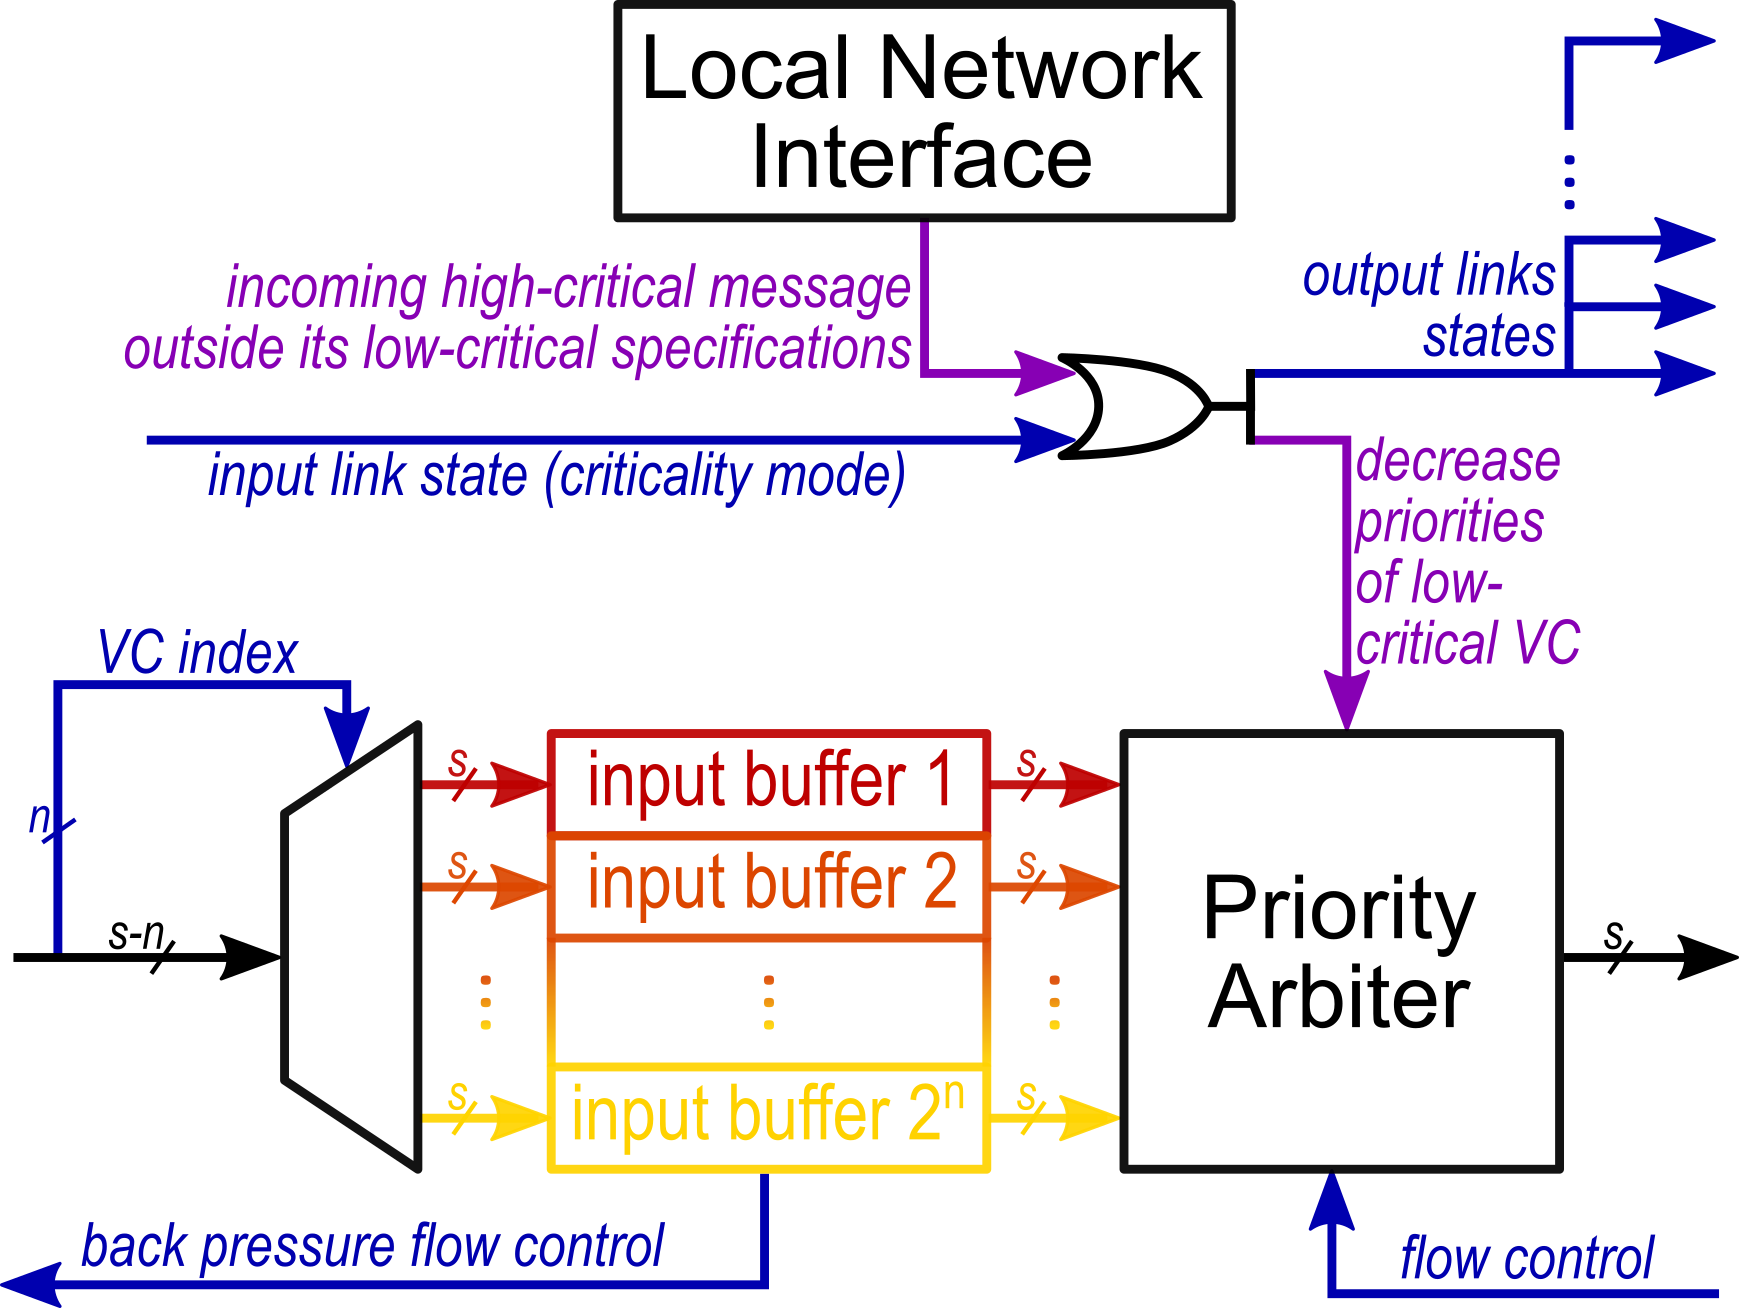
\includegraphics[width=0.8\textwidth]{WPMCFloodRouter.png}
\end{center}
\end{frame}
%%%%%%%%%%%%%%%%%%%%%%%%%%%%%%%%%%%%%%%%%%%%%%%%%%%%%%%
\begin{frame}{Wormhole with Blocking Counter}
\vspace{-0.3cm}
The header flit of critical messages contains a \textit{Blocking Counter} field.
\vspace{1cm}


\includegraphics[width=0.85\textwidth, center]{BC.png}
\end{frame}
%%%%%%%%%%%%%%%%%%%%%%%%%%%%%%%%%%%%%%%%%%%%%%%%%%%%%%%
\begin{frame}{Adaptive Routing}
\begin{columns}

\begin{column}{0.4\textwidth}
\includegraphics<1>[width=0.85\textwidth, right]{AR1.png}
\includegraphics<2>[width=0.85\textwidth, right]{AR2.png}
\end{column}

\begin{column}{0.6\textwidth}
\begin{itemize}
\item <1-> Message BE1\\
Path list : \{(1,2), (2,2)\}, \{(1,2), (1,1), (2,1), (2,2)\}
\vspace{0.5cm}
\item <2-> Message C1\\
Path list: \{(1,2), (2,2)\}
\end{itemize}
\end{column}

\end{columns}
\end{frame}

\begin{frame}{Adaptive Routing - Control Scheme}
\begin{center}
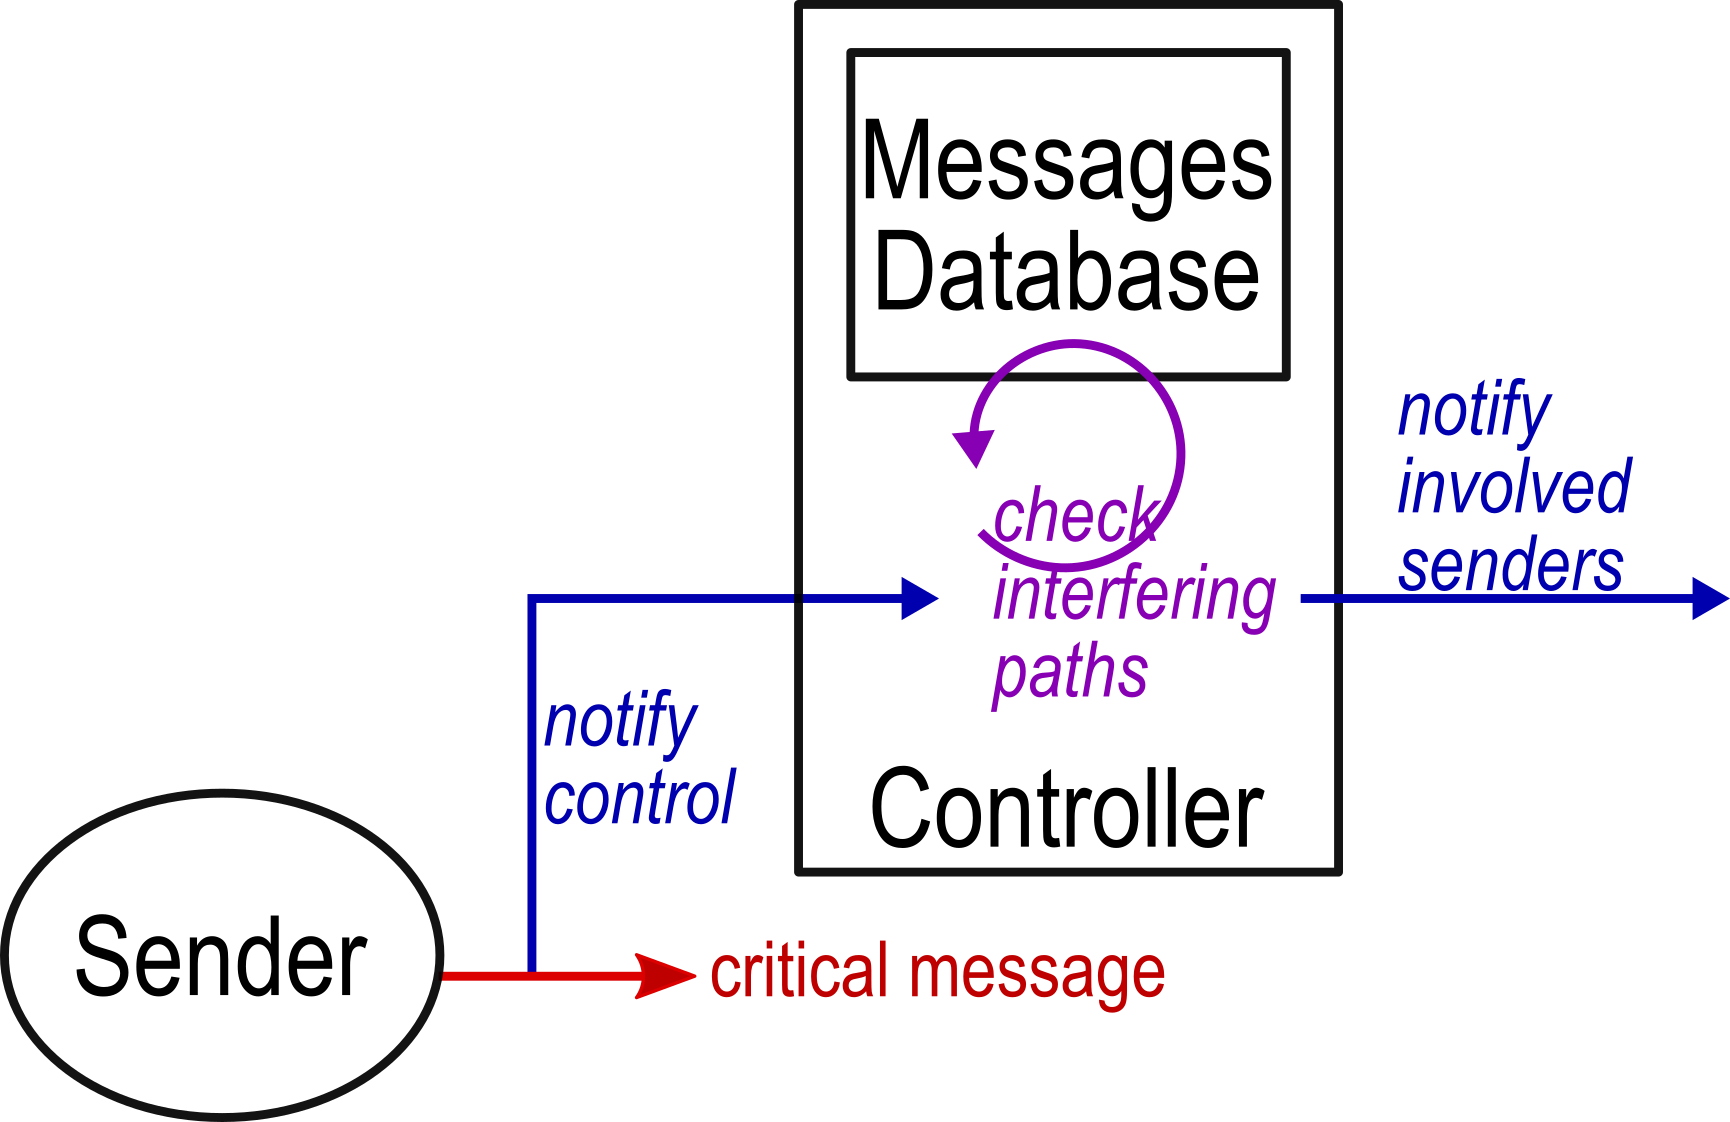
\includegraphics[width=0.75\textwidth]{ARCL.png}
\end{center}

\end{frame}

%%% Local Variables:
%%% mode: latex
%%% TeX-master: "slides"
%%% End:
